\documentclass[10pt, twocolumn]{article}\usepackage[]{graphicx}\usepackage[]{color}
%% maxwidth is the original width if it is less than linewidth
%% otherwise use linewidth (to make sure the graphics do not exceed the margin)
\makeatletter
\def\maxwidth{ %
  \ifdim\Gin@nat@width>\linewidth
    \linewidth
  \else
    \Gin@nat@width
  \fi
}
\makeatother

\usepackage{Sweavel}


\usepackage[breaklinks=true]{hyperref}
\usepackage{url}
\usepackage[a4paper, margin = 1.5cm]{geometry}
\usepackage{a4wide}
\usepackage{float}
\usepackage[english]{babel}
\usepackage[utf8]{inputenc}
\usepackage{amsmath}
\usepackage{amssymb}
\usepackage{xspace}
\usepackage[backend=bibtex,style=numeric-comp,sorting=none]{biblatex}
\bibliography{gia3}
\usepackage{subcaption}
\usepackage[font={small}]{caption}
\usepackage{booktabs}
\usepackage{listings}
\usepackage{cleveref}
\usepackage{lipsum}
\newcommand{\approxtext}[1]{\ensuremath{\stackrel{\text{#1}}{=}}}
\newcommand{\matr}[1]{\mathbf{#1}}
\newcommand{\partt}[2]{\ensuremath{\dfrac{\partial {#1}}{\partial {#2}}}}
\renewcommand{\d}[1]{\ensuremath{\operatorname{d}\!{#1}}} % non-italized differentials
\newcommand{\h}[0]{\ensuremath{\hbar}} % hbar
\def\changemargin#1#2{\list{}{\rightmargin#2\leftmargin#1}\item[]}
\let\endchangemargin=\endlist 
\usepackage{amsthm}
\theoremstyle{plain}
\renewcommand{\theequation}{\thesection.\arabic{equation}}
\def\changemargin#1#2{\list{}{\rightmargin#2\leftmargin#1}\item[]}
\let\endchangemargin=\endlist    
\newcommand{\ts}{\textsuperscript} 
% Stephen's stuff
\newcommand{\R}{\texttt{R}}
\newcommand{\Rfunction}[1]{{\texttt{#1}}}
\newcommand{\Robject}[1]{{\texttt{#1}}}
\newcommand{\Rpackage}[1]{{\mbox{\normalfont\textsf{#1}}}}
\usepackage{xcolor}
\definecolor{Red}{rgb}{0.7,0,0}
\definecolor{Blue}{rgb}{0,0,0.8}
\hypersetup{%
pdfusetitle,
bookmarks = {true},
bookmarksnumbered = {true},
bookmarksopen = {true},
bookmarksopenlevel = 2,
unicode = {true},
breaklinks = {false},
hyperindex = {true},
colorlinks = {true},
linktocpage = {true},
plainpages = {false},
linkcolor = {Blue},
citecolor = {Blue},
urlcolor = {Red},
pdfstartview = {Fit},
pdfpagemode = {UseOutlines},
pdfview = {XYZ null null null}
}
%% Listings
\lstset{ 
language=R,                     % the language of the code
basicstyle=\footnotesize,       % the size of the fonts that are used for the code
numbers=left,                   % where to put the line-numbers
numberstyle=\tiny\color{gray},  % the style that is used for the line-numbers
stepnumber=1,                   % the step between two line-numbers. If it's 1, each line will be numbered
numbersep=5pt,                  % how far the line-numbers are from the code
backgroundcolor=\color{white},  % choose the background color. You must add \usepackage{color}
showspaces=false,               % show spaces adding particular underscores
showstringspaces=false,         % underline spaces within strings
showtabs=false,                 % show tabs within strings adding particular underscores
rulecolor=\color{black},        % if not set, the frame-color may be changed on line-breaks within not-black text (e.g. commens (green here))
tabsize=2,                      % sets default tabsize to 2 spaces
captionpos=b,                   % sets the caption-position to bottom
breaklines=true,                % sets automatic line breaking
breakatwhitespace=false,        % sets if automatic breaks should only happen at whitespace
title=\lstname,                 % show the filename of files included with \lstinputlisting;
% also try caption instead of title
keywordstyle=\color{blue},      % keyword style
commentstyle=\color{green},   % comment style
stringstyle=\color{purple},      % string literal style
escapeinside={\%*}{*)},         % if you want to add a comment within your code
morekeywords={*,...}            % if you want to add more keywords to the set
} 
\usepackage{verbatim}
\usepackage{multicol}
\def\changemargin#1#2{\list{}{\rightmargin#2\leftmargin#1}\item[]}
\let\endchangemargin=\endlist
\addtolength{\oddsidemargin}{-.35in}
\addtolength{\evensidemargin}{-.35in}
\addtolength{\textwidth}{.7in}

%%%%%%%%%%%%%%%%%%%% Begin
\title
{
%\phantom{a}\vspace{2cm}
\textbf
{
Genome Informatics: Assignment 3}\\[1em]
\small{University of Cambridge}
}

\author{Henrik Åhl}
\date{\today}
\renewcommand{\textfraction}{0.05}
\renewcommand{\topfraction}{0.8}
\renewcommand{\bottomfraction}{0.8}
\renewcommand{\floatpagefraction}{0.75}
\makeatletter

\makeatother

\newcommand{\SRY}{\textit{SRY}\xspace}
\newcommand{\HMG}{\textit{HMG}\xspace}
\newcommand{\SOX}{\textit{SOX}\xspace}
\newcommand{\XX}{\textit{XX}\xspace}
\newcommand{\XY}{\textit{X[Y-]}\xspace}
\newcommand{\XYSRY}{\textit{X[Y-]sry}\xspace}
\newcommand{\XYXSRY}{\textit{XXsry}\xspace}
\newcommand{\Y}{\textit{Y}\xspace}

\begin{document}


\date{\today}
\maketitle
\setcounter{page}{1}
\begin{abstract}
%\begin{changemargin}{-.8cm}{-.8cm}
{\bf \SRY is a gene on the \Y chromosome in humans which is significant for sex differentiation primarily in early development. Even though gene expression differences between the sexes are mostly attributed to hormonal differences, we here show that both \SRY and sex chromosome complement carries weight, and importantly, that \SRY only appears to affect gene expression when a \Y chromosome is present. By analysing the human \SRY sequence and transcript to their respective orthologues, and by identifying structurally important parts of the gene, we gain insights into the functionality of \SRY and its effect on expression levels for autosomal genes.  
}
\end{abstract}
\section*{Preface}
This is an assignment report in connection to the \textit{Genome Informatics} module in the Computational Biology course at the University of Cambridge, Michaelmas term 2016. All related code is as of \date{\today} available per request by contacting \href{mailto:hpa22@cam.ac.uk}{hpa22@cam.ac.uk}. Data used is acquired from NCBI's Gene Expression Omnibus, GEO Series Accession number \href{https://www.ncbi.nlm.nih.gov/geo/query/acc.cgi?acc=GSE21822}{GSE21822}. Ortholog and SNP data is supplied by the Ensembl database under the \href{http://www.ensembl.org/Homo_sapiens/Gene/Summary?db=core;g=ENSG00000184895;r=Y:2786855-2787699;t=ENST00000383070}{\SRY} gene information page. For genome related analyses, the GRCh38.p7 version of the human genome was used. 

\section*{Introduction}
In placental mammals and marsupials, sex differentiation is generally determined by the complementary Y chromosome, which is typically linked to testis development and overall commitment to male sexual fate. In humans, this happens primarily because the Y chromosome contains the so-called Sex-determining Region Y (\SRY; also known as the Testis-determining Factor~\cite{tdf}) -- a gene encoding for the likewise named gene-regulatory transcription factor. Also in other mammals, \SRY plays a similar role, and is typically the one signifying gene for differentiation of bipotent organs to the male variants~\cite{riseandfall,bipotent}. 

All orthologs of \SRY are signified by the existence of a specific High-Mobility Group (\HMG)-box, which all tend to be involved in DNA-regulatory processes, such as looping and bending of the structure~\cite{evolsry}. The group as a whole is very prevalent in nature, but the various kinds can be extremely diverse, with conversation of amino acids as low as 50~\% between species~\cite{hmgconserved}. 

The \SRY \HMG-box bases the common reference point for several developmentally important genes entitled \SOX (\textit{S}RY-like HMG-b\textit{ox}) genes, which are named as such precisely because they contain the common \HMG box, but share no other greater similarities because of this. Together, \SRY, which is sometimes referred to as \textit{SoxA}, and the other \SOX genes form the so-called \SOX gene family. \SRY has been proven to be sufficient for testis development, but in the absence of the gene, male sexual fate commitment can still happen in some cases through complementary action of the \SOX-\textit{9} gene~\cite{soximportance,sox9}. 
% autosomal -- not sex

We here investigate the structural features of \SRY in humans and its orthologs and attempt to assess differences and similarities. We also, in imitation of Wijchers et al.~\cite{complement}, show that \SRY is not the sole driving factor of differential expression in autosomal genes, but that also the sex chromosome complement is important. More precisely, our results indicate that \SRY acts collaboratively with the \textit{Y} chromosome in order to induce differential expression in a set of autosomal genes.

\section*{Methods}
Using the given approach in \cite{complement}, we analyse our raw cDNA from a hybridization to Affymetrix mouse genome 430 2.0. As samples, we have four different genotypes, consisting of sex chromosome setups \XX, \XYSRY, \XY and \XYSRY. The two prior represent individuals with  male phenotypical characteristics, and the two latter the female counterparts. The chromosomal setups with the \textit{sry} suffix are named as such because they have had an \SRY transgene inserted into an autosome. Similarly, \textit{[Y-]} represents Y chromosome variants that have been modified to not contain the \SRY gene~\cite{y-}. For every chromosomal setup, there are three biological replicates, where all individual data is gathered from earpunches of the specimen involved. 

According to the authors in our study of interest, the Bioconductor \texttt{RMA} package in \R~is used for preprocessing of the raw .CEL files. However, no such package appears to exist~\cite{biocpackages}. Because of this discrepancy, we in this investigation use the Bioconductor \texttt{affy} package for preprocessing, using the default \textit{rma} function with quantile normalisation and RMA background correction. Like the authors, we define differential expression as being greater or equal than a log-2 fold change of 1.2, as well as fulfilling a Student's T-test with $p < 0.05$). This we do using the \texttt{simpleaffy} package, along with quality-control by \texttt{affyQCreport}. In addition, we also filter probes using MAS5.0 absent/present calls. 

Orthologues to \SRY are taken from Chimpanzee, Cow, Macaque, Mouse, Pig (two genes), Rat and Vervet-AGM. For alignment of the these genes and their transcripts we use Clustal Omega 1.2.3 and MUSCLE 3.8 respectively. Motif identification and analysis is done with Meme-suite 4.11.2 modules MEME, Tomtom and MAST. 

\section*{Results}





\subsection*{Gene expression hints at collaborative action between \SRY and the \Y chromosome}
In the quality control of our samples, no clear discrepancies can be determined to be present. We therefore choose to keep all samples for our analyses.

To determine whether sex-chromosome sensitivity (SCS) affects autosomal gene expression over the whole genome, we produce the comparison seene in \cref{fig:venns}A and B where differences between the genotypes of the males (A) and females (B) are shown. Using our definition of significant expression values, we are able to round up 126 SCS genes, as opposed to Wijchers et al.\ who find 369 differentially expressed genes under the same conditions. Nevertheless, we are able to produce the same trends in the expression, namely that our SCS genes are biased towards an \XX configuration at its core in males, and the contrary in females. Similarly, we establish a set of sex-sensitive and dimorphic genes (SSD) comparing \XX and \XYSRY individuals, and are able to find a selection of 46 (175) such genes. We also identify 287 (401) diti in either sex. A list of the genes contained in each group can be provided upon request.

We can furthermore see hints of the effects of \SRY in \cref{fig:expression}D and E. Notably, in the \textit{XY} comparison, \SRY introduces a trend towards the samples without the transgene, whereas in our \XX samples the opposite happens. However, the difference in subfigure E is significantly smaller, suggesting that the \SRY acts collaboratively with the \Y complement, i.e.\ we have an effect from \SRY primarily when we also have the \Y chromosome. It is also evident that some genes have clear preferences towards the \Y chromosome (cf.\ the outliers in \cref{fig:expression}A, B, C, F), giving fairly constant differential expressions between the comparisons, and subsequently not being affected categorically by the presence of \SRY. Because of these results we converge on our previously mentioned set of sex sensitive dimorphic genes (see \cref{fig:venns}B) in determining the effects caused solely by our transgene.

When instead limiting our analysis to our new set of genes, we see from the blue triangles in \cref{fig:expression}D and E that the effect from \SRY has vanished. We nonetheless retain that a part our genes are being affected mostly by the sex chromosome, most notable seen in \cref{fig:expression}C and F. Again, we also see that the trend shift for most of the SSD genes only occurs when \SRY is put in combination with the \Y chromosome.

\begin{Schunk}
\begin{figure}[H]

{\centering \includegraphics[width=\maxwidth]{figure/twocolumn-venns-1} 

}

\caption[Venn representations of genes differentially expressed in various groups of interest, and their corresponding overlaps]{Venn representations of genes differentially expressed in various groups of interest, and their corresponding overlaps.}\label{fig:venns}
\end{figure}
\end{Schunk}

\subsection*{\SRY is poorly conserved apart from the \HMG-box structure}
In doing sequence alignments of \SRY and its orthologues, we find that the sequences differ significantly, with almost no conservation of the overall structure. The one conserved structure is the region coding for the transcript \HMG-box; when mapping the human \SRY \HMG-box to the 9 orthologues the result is a ca. 90~\% identity in the (non-fragmented) \HMG-box region. In contrast, when only the gene sequences are set to match against each other, they do so with ca. 70~\% conservation in the same region. The transcripts perform slightly better with ca.\ 85~\% complete or near global match. Alignments can be provided upon request.

When piped through motif detection and analysis software, the conserved and matched motifs typically either correspond to other \SOX genes or indeed \HMG-boxes, further establishing the notion of the \HMG-box being the structurally most significant part of the gene and transcript. It also suggests that the gene is first and foremost modulatory, i.e. having the role of binding to parts of the DNA and structurally affecting it in various ways. 

By analysing SNP data, we find that point mutations which gives rise to disease or a phenotypic change are focused to the \HMG-box region in humans. This can be seen in figure~\cref{fig:snp}. Other SNPs (not shown here) are still concentrated towards the region, although a far greater amount of mutations are distributed outside of this area. 

\begin{Schunk}
\begin{figure}[H]

{\centering 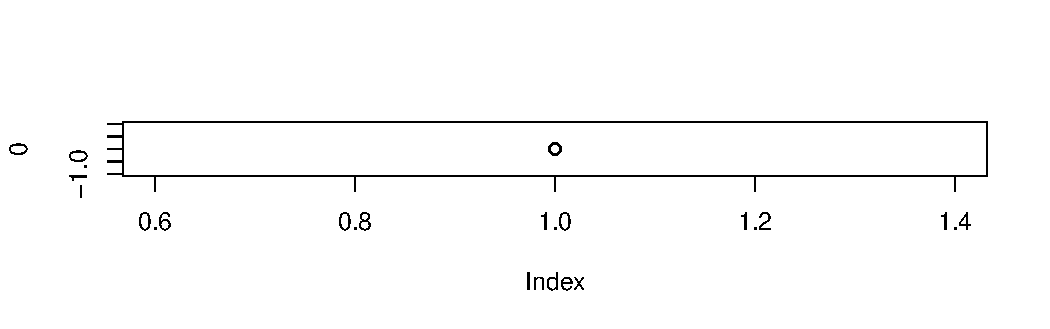
\includegraphics[width=\maxwidth]{figure/twocolumn-snp-1} 

}

\caption[Known SNPs related to disease or changes in phenotype]{Known SNPs related to disease or changes in phenotype. Axis shows chromosome coordinates.}\label{fig:snp}
\end{figure}
\end{Schunk}

\section*{Discussion}
Analysing the sequence and its structural traits hints at \SRY indeed being mostly modular, and functionally revolving around its ability to bind to and affect DNA structure. Also the SNP investigations reinforce this, as it appears as the transcript to a higher degree tends  be lost or malfunctioning when the modulatory region is altered.

Our expression analysis shows that, in addition to being regulated by \SRY, a fair amount of genes are dependent primarily on the sex chromosome complement. In addition, we see that the genes being affected in their expression mostly by \SRY in fact only appear to be so when there is also a \Y chromosome prevalent, and interestingly enough almost exclusively in a repressive manner. Further investigations are clearly required, but even from our analysis it appears plausible that some genes are driven mostly by chromosomal complement, whereas some instead are directly or indirectly repressed by \SRY. Importantly, it appears as if the modulatory significance of the \SRY transcript is mainly in relation to the parts of the \Y chromosome, and seemingly not a genome-wide phenomenon. Because of the repressive effect, it could be the case that \SRY hampers transcription of genes directly through its structurally affecting role, but this phenomenon could also be indirect; further analysis is needed.

The differences in genes sensitive to our different variables ought to be mainly because of the seemingly different approach in preprocessing of the data. Still, this gives us relatively different results in considering the effects of \SRY, as we see an effect related to the transgene in addition to just the sex-sensitivity, which is the result of the authors. Other results are difficult to compare due to the representation of the data points found in the reference paper, as the authors have chosen to visualize the set on top of the subset and thus effectively preventing an accurate comparison.

Our results here have given a further insight into the impact of \SRY with respect to autosomal gene expression, and suggested that \SRY might work collaboratively with the \Y chromosome in order to affect this. Ultimately, more rigorous studies on \SRY transcript targets and functionality is naturally what can help unravel the true nature of these results.

\section*{Acknowledgements}
As always, many thanks to Julian Melgar for no particular reason. Also thanks to Klara Berg for proofreading.

%\newpage
\printbibliography

\begin{Schunk}
\begin{figure*}[h]

{\centering \includegraphics[width=\maxwidth]{figure/twocolumn-expression-1} 

}

\caption{Pairwise comparisons between log-2 gene expression values of the four core chromosomal pairs. The dashed lines represent a log-2 fold change of 1.2. Red dots represent the SCS genes, whereas the blue triangles correspond to the sex-chromosome sensitive \textit{XY} dimorphic genes. Note how subfigures \textbf{A}, \textbf{B} and \textbf{C} are involved in determining the sets of SCS and SSD genes (see \cref{fig:venns}).}\label{fig:expression}
\end{figure*}
\end{Schunk}

\end{document}
